\subsection{Stacking Ensemble}\label{subsec:stacking_ensemble}
Given the results of the optimization process, we implemented a stacking ensemble to combine the predictions of the top-performing configurations.
As with all our experiments, we follow the procedure outlined in Section~\ref{subsec:validation_testing_procedures} to evaluate the performance of the stacking ensemble.

For each oxide, we first identified the top-performing configurations to use in the stacking ensemble.
To identify the top-performing configurations for use in the stacking ensemble, we developed a category-based method that groups models into distinct categories for systematic comparison.
This approach helps in selecting models that perform optimally for specific tasks while ensuring diversity within the ensemble.
Additionally, we developed and employed a grid search to identify the optimal ensemble configurations, but time constraints prevented us from fully completing this process.
Finally, we employed the stacking model and evaluated its performance.
We present the results as well as the 1:1 plots in Section~\ref{subsec:stacking_ensemble_results}.

\subsubsection{Category Method \& Pipeline Selection}\label{subsec:category_method}
The category-based method organizes models into the following groups:

\begin{itemize}
    \item Gradient Boosting: \gls{gbr}, \gls{xgboost}, \gls{ngboost}
    \item Tree-Based: \gls{etr}, \gls{rf}
    \item Linear and Regularized Models: \gls{lasso}, Ridge, \gls{enet}
    \item SVM: \gls{svr}
    \item PLS: \gls{pls}
\end{itemize}

We used the top-performing configurations identified in Section~\ref{sec:optimization_results} to select configurations for the stacking ensemble.

For each oxide, we filtered the trial data from the optimization experiment to create a dataset containing configuration information and performance metrics.
These datasets were sorted by \gls{rmsecv}.
We then selected unique model types for further analysis, based on the categories above.
Our process involved selecting a set number of configurations for each category until a maximum number of configurations for the oxide's ensemble was reached.

To ensure diversity and limit scope, we set a maximum of one model per category and three models per stacking ensemble, with one ensemble for each oxide.
For each oxide, we developed pipelines to preprocess the data according to the given configuration and to utilize the models with their optimal hyperparameters.
These pipelines represent the optimal configurations for each oxide, and are used as base estimators in the stacking ensemble.

\subsubsection{Grid Search}\label{subsec:grid_search}
The grid search process begins by generating all possible combinations of the selected models.
Specifically, we generate combinations with at least two models, up to a configurable maximum number of models.

For each oxide, we constructed a pipeline for each of the top model configurations identified in Section~\ref{sec:optimization_results}.
The evaluation function iterates over each combination of base estimators, constructs a stacking ensemble pipeline, and assesses its performance using cross-validation.

The evaluation function prepares the pipeline with the current combination of base estimators and splits the data into training and testing sets using our data partitioning method.
The stacking ensemble is then fitted on the training set, and the meta-features generated from the base estimators are used to train the final estimator.

We compute the evaluation metrics to assess the ensemble's effectiveness.
The best combination is identified based on the lowest \gls{rmsecv} value.

It is possible to vary the meta-learner in this process, adding another variable to tune as part of the search process.

While our grid search implementation was limited to the \ce{TiO2} oxide, the methodology demonstrates the potential for identifying optimal stacking ensembles by systematically evaluating model combinations and their configurations.
We chose not to pursue this method further due to the time constraints of this project, but believe it is a promising approach for future work.


\subsubsection{Results}\label{subsec:stacking_ensemble_results}
For each major oxide, we ran the stacking ensemble and evaluated its performance.
The evaluations were conducted using the same configurations, varying only the meta-learner between runs.
We present the results for the \gls{enet} meta-learner with \texttt{alpha} = 1.0, as well as for the \gls{enet} meta-learner with \texttt{alpha} = 0.1.
Additionally, we present the results for the \gls{svr} meta-learner, using the default hyperparameters provided by \texttt{scikit-learn}.

The evaluation metrics are shown in Table~\ref{tab:stacking_ensemble_results_enet}, Table~\ref{tab:stacking_ensemble_results_enet_01}, and Table~\ref{tab:stacking_ensemble_results_svr}.
Additionally, we provide 1:1 plots for each ensemble in Figures~\ref{fig:elasticnet_one_to_one}, \ref{fig:enetalpha01_one_to_one}, and \ref{fig:svr_one_to_one}, showing the actual versus predicted values for each oxide.

A notable observation from our results is that different meta-learners exhibited varying performance levels across oxides.
We observed that the final predictions were strongly affected by the meta-learner, going as far as rendering some predictions nonsensical if the wrong meta-learner was chosen.
Specifically, for \ce{TiO2}, we observed that predictions remained near-constant values despite varying the combination of model configurations in the \ce{TiO2} ensemble.
In fact, this was the reason for our implementation of the grid search process.
The consistency of our observations supported our hypothesis: changing only the meta-learner significantly impacts the \gls{rmsecv} and prediction outcomes.
We decided to investigate further and identified potential issues with small value predictions when using an \gls{enet} meta-learner.
For example, most values for \ce{TiO2} fell between 0 and 2.5, as shown in Figure~\ref{fig:oxide_distributions}.
The regularization term likely dominated the fitting process, leading to underfitting and resulting in nearly constant predictions.
This hypothesis was confirmed by adjusting the regularization parameter, \texttt{alpha}, in the \gls{enet}.
Lowering \texttt{alpha} produced better outcomes, indicating that regularization adversely affected the predicted values.
The 1:1 plot in Figure~\ref{fig:elasticnet_one_to_one} shows the near-constant predictions for \ce{TiO2} when using a \gls{enet} meta-learner, and Figure~\ref{fig:enetalpha01_one_to_one} shows the improved predictions with \texttt{alpha} = 0.1.
This leads us to conclude that the meta-learner's choice significantly impacts the \gls{rmsecv} and prediction outcomes.

The stacking approach demonstrated strong improvements in prediction accuracy compared to the baseline described in Section~\ref{sec:baseline_replica}, validating the efficacy of our methodology.
We measured this improvement using \gls{rmsep}, which provides the fairest comparison between the baseline and the stacking approach.
As mentioned, \gls{rmsep} evaluates the model's performance on the test set.
In Section~\ref{sec:baseline_replica}, we described how the baseline test set was constructed by sorting extreme concentration values into the training set, and then performing a random split.
As noted in Section~\ref{subsec:validation_testing_procedures}, a more sophisticated procedure is required to support the testing and validation strategy in this work.
Despite the differences in test set construction, the test sets remained similar in composition\footnote{The analysis of this can be found on our GitHub repository: \url{https://github.com/chhoumann/thesis-chemcam}}, which allowed us to use \gls{rmsep} as a fair comparison metric.
Table~\ref{tab:stacking_ensemble_vs_moc} compares the \gls{rmsep} values of different oxides for the \gls{moc} (replica) model with three stacking ensemble models: \gls{enet} with $\alpha = 1$, \gls{enet} with $\alpha = 0.1$, and \gls{svr}.
Overall, the stacking ensemble models tend to produce lower \gls{rmsep} values compared to the \gls{moc} (replica) model.
Notably, \ce{SiO2}, \ce{TiO2}, \ce{Na2O}, and \ce{K2O} show large improvements across all stacking ensemble models.
For instance, the \gls{rmsep} for \ce{SiO2} is reduced from 5.61 (\gls{moc} (replica)) to around 3.59 (\gls{enet} with $\alpha = 1$) and further to 3.47 (\gls{svr}).
Similarly, \ce{TiO2} shows a reduction from 0.61 (\gls{moc} (replica)) to 0.32 (\gls{enet} with $\alpha = 0.1$).
The improvements are consistent across most oxides, with \gls{enet} and \gls{svr} models both outperforming the \gls{moc} (replica) model.
This shows that the ensemble approach, particularly with these meta-learners, enhances prediction accuracy for the oxides we tested.

The results presented above indicate a strong performance from the stacking ensemble approach.
However, it is important to note that some evaluation metrics are worse in the stacking approach than in certain individual configurations.
We believe that further tuning, particularly of the meta-learner's hyperparameters, could substantially improve these results.

\begin{table}
\centering
\caption{Stacking ensemble results using the \gls{enet} model as the meta-learner with $\alpha = 1$.}
\begin{tabular}{lcccc}
\toprule
Oxide          & \gls{rmsep} & STDDEV & \gls{rmsecv}         & Std. Dev. CV          \\
\midrule
\ce{SiO2}      & 3.588       & 3.582  & 4.680 $\pm$ 0.500    & 4.670 $\pm$ 0.516     \\
\ce{TiO2}      & 0.571       & 0.565  & 0.818 $\pm$ 0.111    & 0.814 $\pm$ 0.117     \\
\ce{Al2O3}     & 1.656       & 1.657  & 2.211 $\pm$ 0.023    & 2.199 $\pm$ 0.226     \\
\ce{FeO_T}     & 1.794       & 1.789  & 2.792 $\pm$ 0.649    & 2.745 $\pm$ 0.646     \\
\ce{MgO}       & 0.711       & 0.711  & 1.660 $\pm$ 0.525    & 1.635 $\pm$ 0.516     \\
\ce{CaO}       & 1.636       & 1.619  & 1.307 $\pm$ 0.205    & 1.290 $\pm$ 0.202     \\
\ce{Na2O}      & 0.470       & 0.462  & 1.075 $\pm$ 0.706    & 1.067 $\pm$ 0.710     \\
\ce{K2O}       & 0.476       & 0.462  & 0.653 $\pm$ 0.195    & 0.652 $\pm$ 0.193     \\
\bottomrule
\end{tabular}
\label{tab:stacking_ensemble_results_enet}
\end{table}

\begin{table}
\centering
\caption{Stacking ensemble results using the \gls{enet} model as the meta-learner with $\alpha = 0.1$.}
\begin{tabular}{lcccc}
\toprule
Oxide          & \gls{rmsep} & STDDEV & \gls{rmsecv}         & Std. Dev. CV          \\
\midrule
\ce{SiO2}      & 3.598       & 3.591  & 4.686 $\pm$ 0.489    & 4.677 $\pm$ 0.505     \\
\ce{TiO2}      & 0.319       & 0.310  & 0.450 $\pm$ 0.083    & 0.448 $\pm$ 0.083     \\
\ce{Al2O3}     & 1.658       & 1.660  & 2.192 $\pm$ 0.235    & 2.180 $\pm$ 0.238     \\
\ce{FeO_T}     & 1.841       & 1.840  & 2.781 $\pm$ 0.664    & 2.731 $\pm$ 0.659     \\
\ce{MgO}       & 0.768       & 0.768  & 1.632 $\pm$ 0.531    & 1.608 $\pm$ 0.518     \\
\ce{CaO}       & 1.647       & 1.627  & 1.310 $\pm$ 0.213    & 1.291 $\pm$ 0.211     \\
\ce{Na2O}      & 0.442       & 0.433  & 1.093 $\pm$ 0.690    & 1.079 $\pm$ 0.692     \\
\ce{K2O}       & 0.494       & 0.477  & 0.556 $\pm$ 0.155    & 0.553 $\pm$ 0.153     \\
\bottomrule
\end{tabular}
\label{tab:stacking_ensemble_results_enet_01}
\end{table}

\begin{table}
\centering
\caption{Stacking ensemble results using the \gls{svr} model as the meta-learner with default hyperparameters.}
\begin{tabular}{lcccc}
\toprule
Oxide          & \gls{rmsep} & STDDEV & \gls{rmsecv}         & Std. Dev. CV          \\
\midrule
\ce{SiO2}      & 3.473       & 3.478  & 5.064 $\pm$ 0.932    & 5.061 $\pm$ 0.926     \\
\ce{TiO2}      & 0.340       & 0.333  & 0.442 $\pm$ 0.087    & 0.442 $\pm$ 0.087     \\
\ce{Al2O3}     & 1.729       & 1.732  & 2.285 $\pm$ 0.226    & 2.274 $\pm$ 0.233     \\
\ce{FeO_T}     & 1.693       & 1.681  & 4.821 $\pm$ 1.490    & 4.768 $\pm$ 1.495     \\
\ce{MgO}       & 0.819       & 0.820  & 2.569 $\pm$ 1.274    & 2.559 $\pm$ 1.271     \\
\ce{CaO}       & 1.594       & 1.574  & 1.475 $\pm$ 0.294    & 1.456 $\pm$ 0.304     \\
\ce{Na2O}      & 0.369       & 0.368  & 0.978 $\pm$ 0.885    & 0.971 $\pm$ 0.887     \\
\ce{K2O}       & 0.511       & 0.497  & 0.669 $\pm$ 0.199    & 0.666 $\pm$ 0.196     \\
\bottomrule
\end{tabular}
\label{tab:stacking_ensemble_results_svr}
\end{table}

\begin{figure*}
    \centering
    \resizebox{0.75\textwidth}{!}{
        \begin{tabular}{cc}
            \begin{subfigure}{0.5\textwidth}
                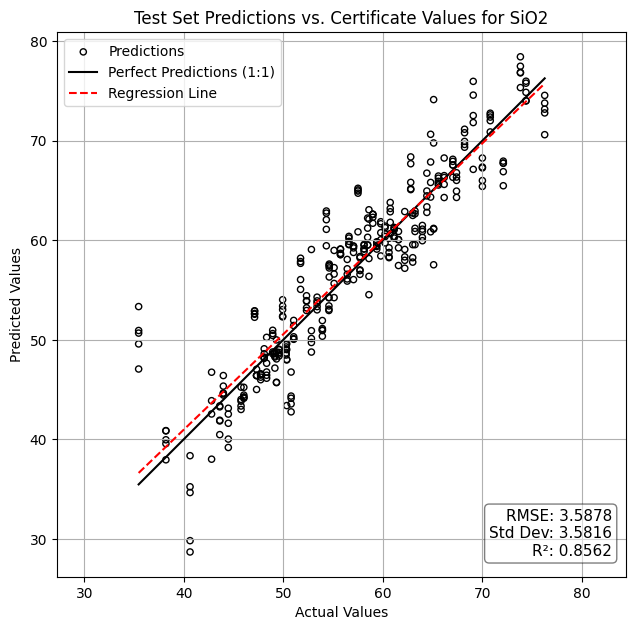
\includegraphics[width=\textwidth]{images/one_to_one/elasticnet/SiO2.png}
            \end{subfigure} & \hspace{3cm}
            \begin{subfigure}{0.5\textwidth}
                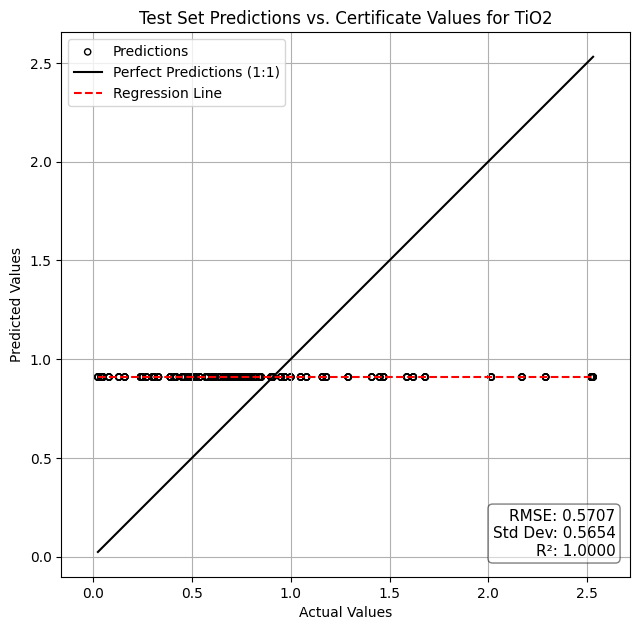
\includegraphics[width=\textwidth]{images/one_to_one/elasticnet/TiO2.png}
            \end{subfigure} \\
            \begin{subfigure}{0.5\textwidth}
                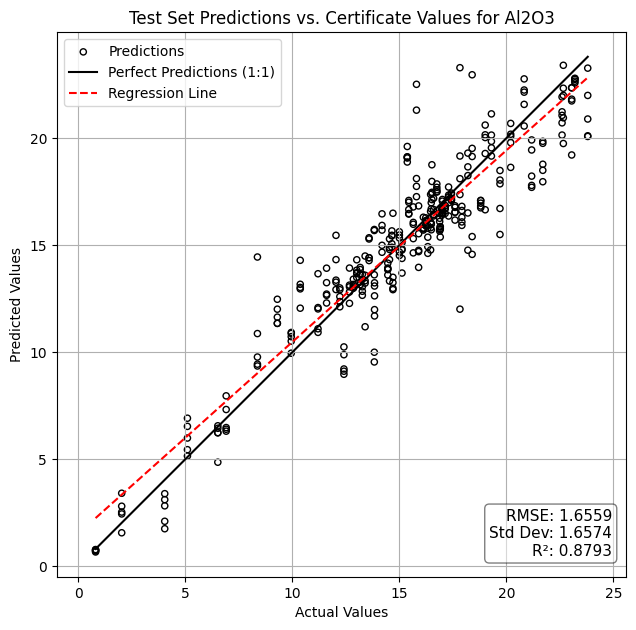
\includegraphics[width=\textwidth]{images/one_to_one/elasticnet/Al2O3.png}
            \end{subfigure} & \hspace{3cm}
            \begin{subfigure}{0.5\textwidth}
                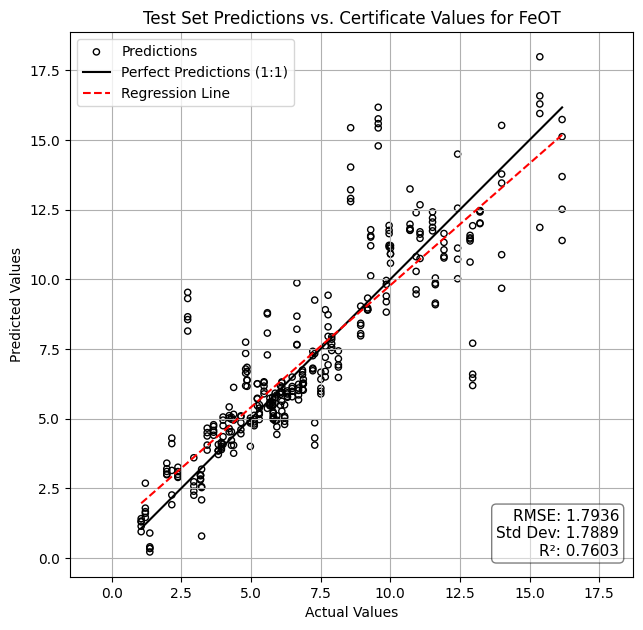
\includegraphics[width=\textwidth]{images/one_to_one/elasticnet/FeOT.png}
            \end{subfigure} \\
            \begin{subfigure}{0.5\textwidth}
                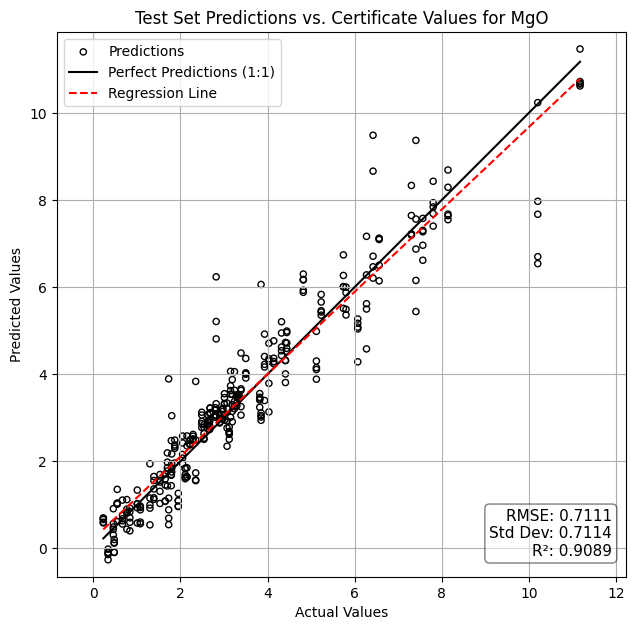
\includegraphics[width=\textwidth]{images/one_to_one/elasticnet/MgO.png}
            \end{subfigure} & \hspace{3cm}
            \begin{subfigure}{0.5\textwidth}
                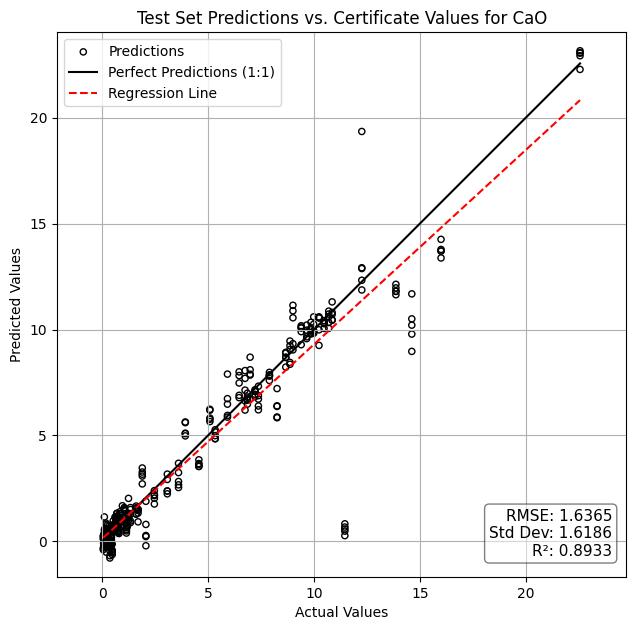
\includegraphics[width=\textwidth]{images/one_to_one/elasticnet/CaO.png}
            \end{subfigure} \\
            \begin{subfigure}{0.5\textwidth}
                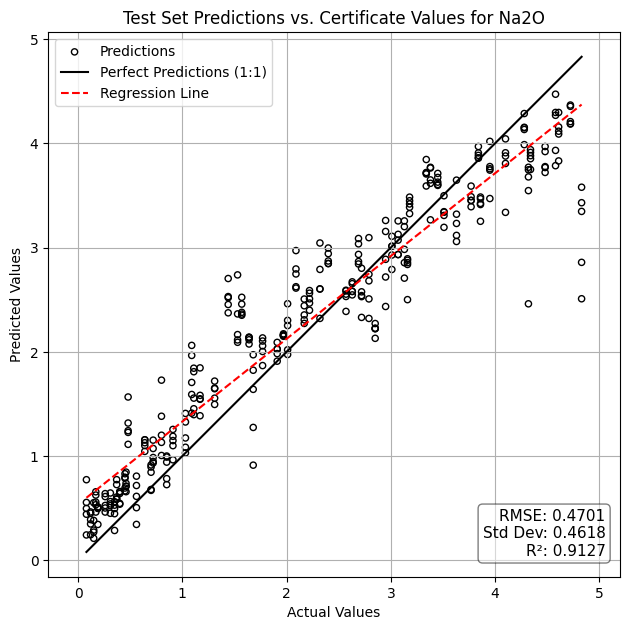
\includegraphics[width=\textwidth]{images/one_to_one/elasticnet/Na2O.png}
            \end{subfigure} & \hspace{3cm}
            \begin{subfigure}{0.5\textwidth}
                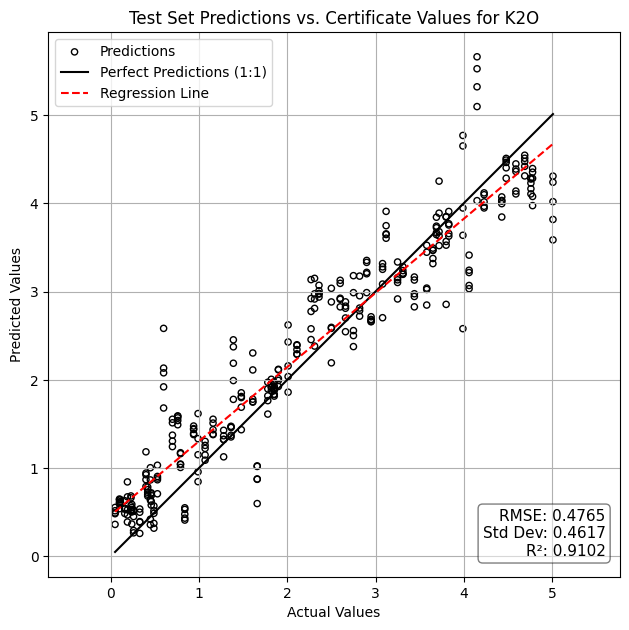
\includegraphics[width=\textwidth]{images/one_to_one/elasticnet/K2O.png}
            \end{subfigure}
        \end{tabular}
    }
    \caption{One-to-one plots for the stacking ensemble model with the \gls{enet} as the meta-learner with $\alpha = 1$}
    \label{fig:elasticnet_one_to_one}
\end{figure*}

\begin{table}
\centering
\caption{Comparison of \gls{rmsep} values for the \gls{moc} (replica) model and various stacking ensemble models.}
\resizebox{0.45\textwidth}{!}{
\begin{tabular}{lccccc}
\toprule
Oxide          & \gls{moc} (replica) & \gls{enet} ($\alpha = 1$) & \gls{enet} ($\alpha = 0.1$) & \gls{svr} \\
\midrule
\ce{SiO2}      & 5.61          & 3.59              & 3.60                & \textbf{3.47} \\
\ce{TiO2}      & 0.61          & 0.57              & \textbf{0.32}       & 0.34 \\
\ce{Al2O3}     & 2.47          & \textbf{1.66}     & 1.66                & 1.73 \\
\ce{FeO_T}     & 1.82          & 1.79              & 1.84                & \textbf{1.69} \\
\ce{MgO}       & 1.56          & \textbf{0.71}     & 0.77                & 0.82 \\
\ce{CaO}       & 2.09          & \textbf{1.64}     & 1.65                & 1.59 \\
\ce{Na2O}      & 1.33          & 0.47              & 0.44                & \textbf{0.37} \\
\ce{K2O}       & 1.91          & \textbf{0.48}     & 0.49                & 0.51 \\
\bottomrule
\end{tabular}
}
\label{tab:stacking_ensemble_vs_moc}
\end{table}

\begin{figure*}
    \centering
    \resizebox{0.75\textwidth}{!}{
        \begin{tabular}{cc}
            \begin{subfigure}{0.5\textwidth}
                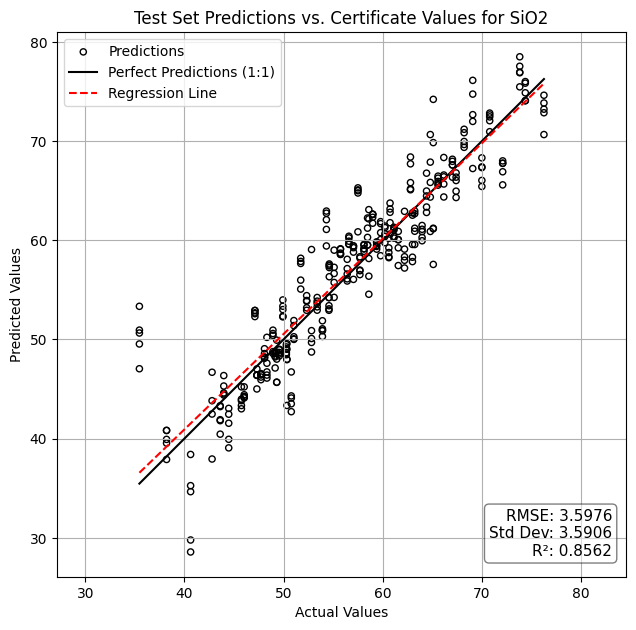
\includegraphics[width=\textwidth]{images/one_to_one/enetalpha01/SiO2.png}
            \end{subfigure} & \hspace{3cm}
            \begin{subfigure}{0.5\textwidth}
                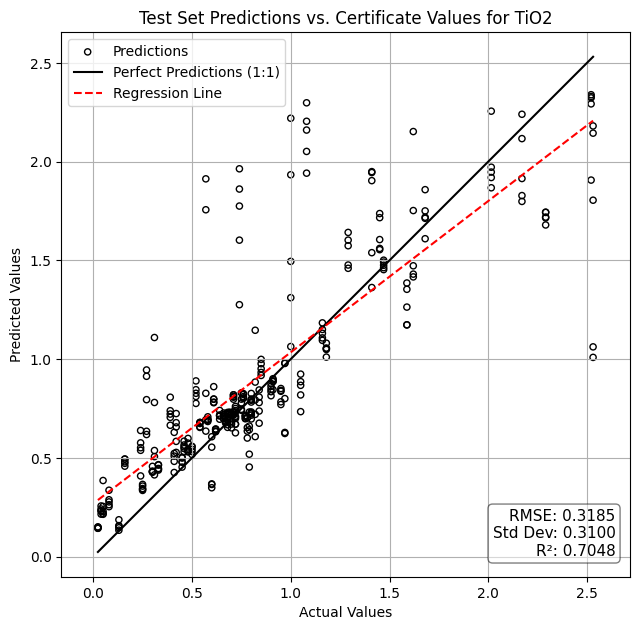
\includegraphics[width=\textwidth]{images/one_to_one/enetalpha01/TiO2.png}
            \end{subfigure} \\
            \begin{subfigure}{0.5\textwidth}
                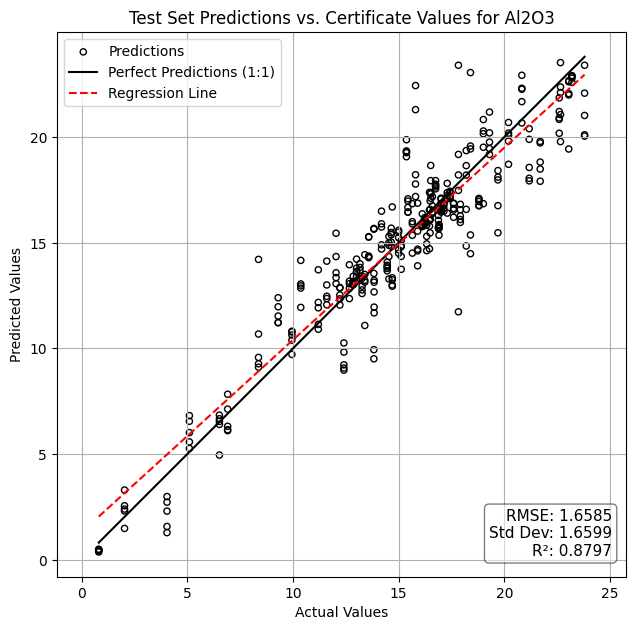
\includegraphics[width=\textwidth]{images/one_to_one/enetalpha01/Al2O3.png}
            \end{subfigure} & \hspace{3cm}
            \begin{subfigure}{0.5\textwidth}
                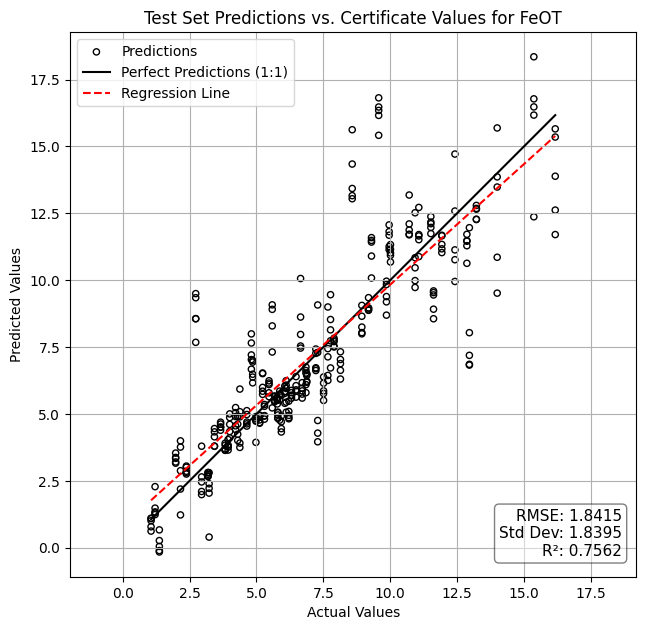
\includegraphics[width=\textwidth]{images/one_to_one/enetalpha01/FeOT.png}
            \end{subfigure} \\
            \begin{subfigure}{0.5\textwidth}
                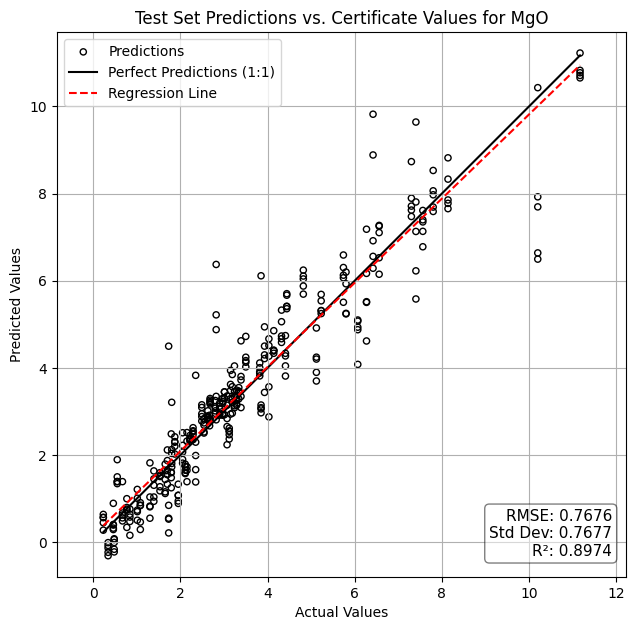
\includegraphics[width=\textwidth]{images/one_to_one/enetalpha01/MgO.png}
            \end{subfigure} & \hspace{3cm}
            \begin{subfigure}{0.5\textwidth}
                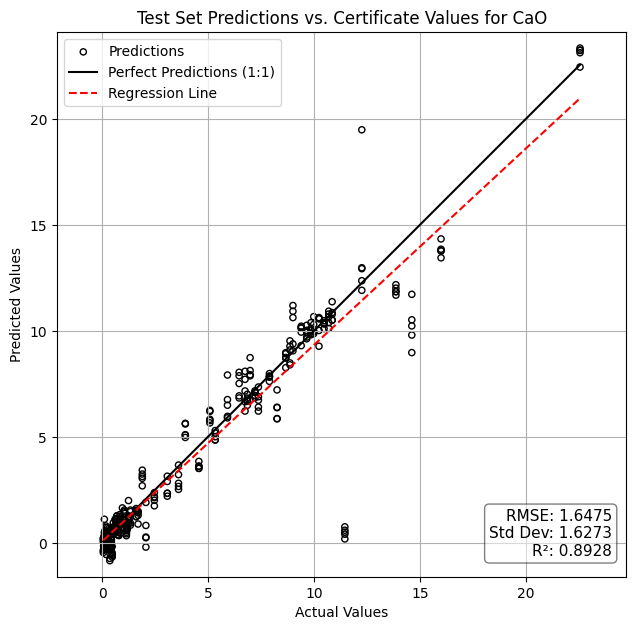
\includegraphics[width=\textwidth]{images/one_to_one/enetalpha01/CaO.png}
            \end{subfigure} \\
            \begin{subfigure}{0.5\textwidth}
                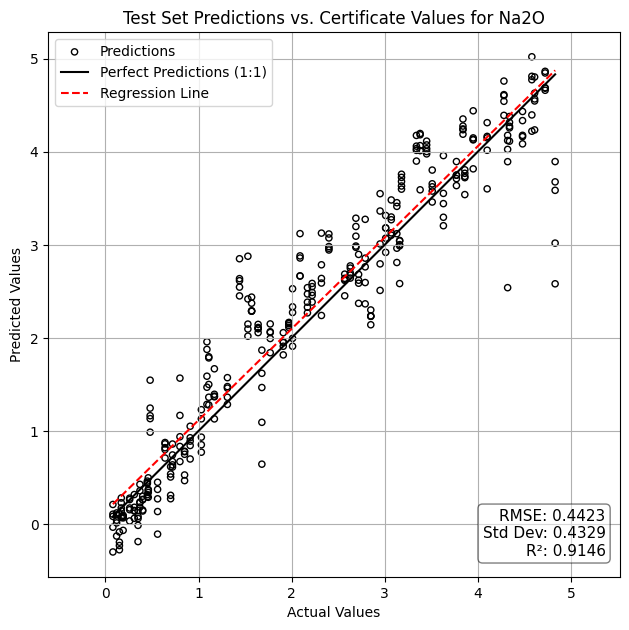
\includegraphics[width=\textwidth]{images/one_to_one/enetalpha01/Na2O.png}
            \end{subfigure} & \hspace{3cm}
            \begin{subfigure}{0.5\textwidth}
                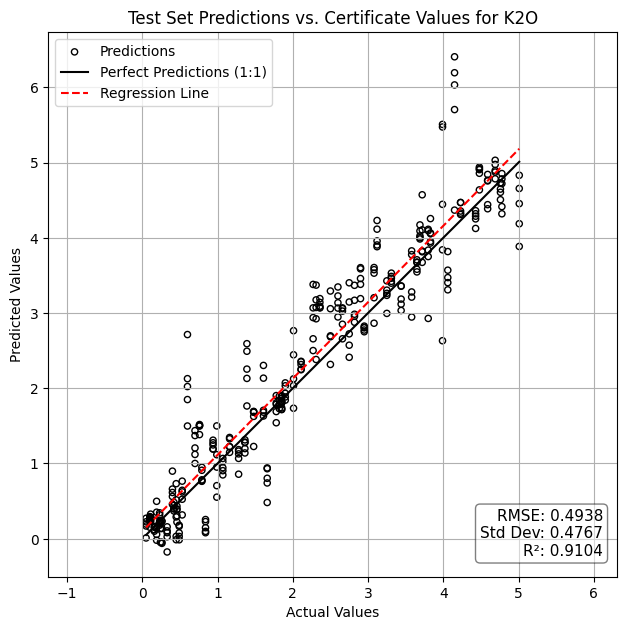
\includegraphics[width=\textwidth]{images/one_to_one/enetalpha01/K2O.png}
            \end{subfigure}
        \end{tabular}
    }
    \caption{One-to-one plots for the stacking ensemble model with the \gls{enet} as the meta-learner with $\alpha = 0.1$.}
    \label{fig:enetalpha01_one_to_one}
\end{figure*}

\begin{figure*}
    \centering
    \resizebox{0.75\textwidth}{!}{
        \begin{tabular}{cc}
            \begin{subfigure}{0.5\textwidth}
                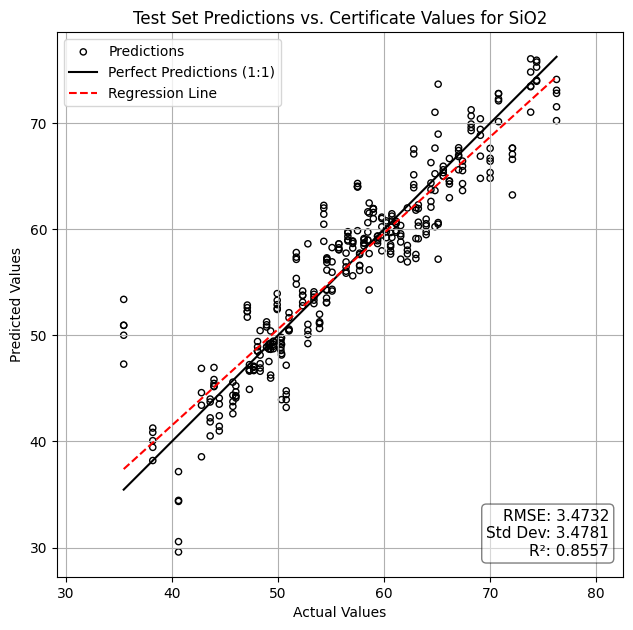
\includegraphics[width=\textwidth]{images/one_to_one/svr/SiO2.png}
            \end{subfigure} & \hspace{3cm}
            \begin{subfigure}{0.5\textwidth}
                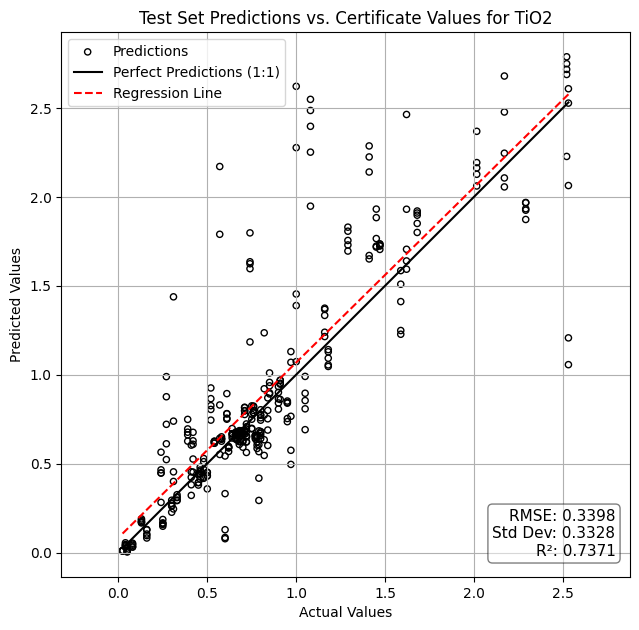
\includegraphics[width=\textwidth]{images/one_to_one/svr/TiO2.png}
            \end{subfigure} \\
            \begin{subfigure}{0.5\textwidth}
                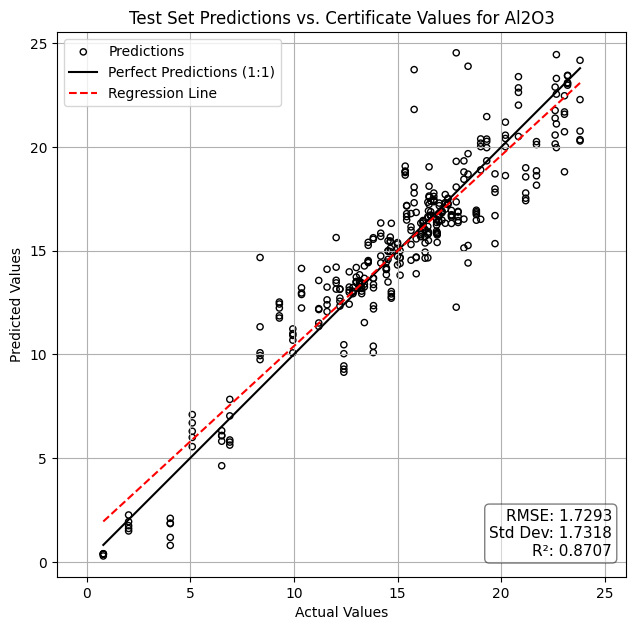
\includegraphics[width=\textwidth]{images/one_to_one/svr/Al2O3.png}
            \end{subfigure} & \hspace{3cm}
            \begin{subfigure}{0.5\textwidth}
                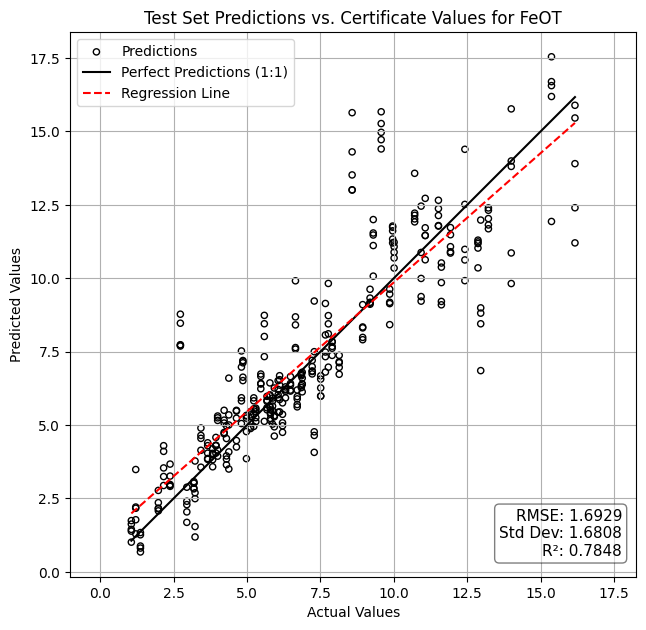
\includegraphics[width=\textwidth]{images/one_to_one/svr/FeOT.png}
            \end{subfigure} \\
            \begin{subfigure}{0.5\textwidth}
                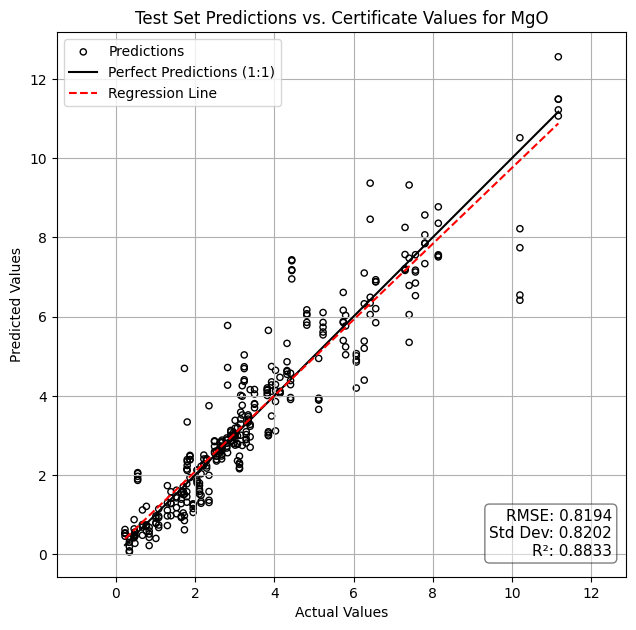
\includegraphics[width=\textwidth]{images/one_to_one/svr/MgO.png}
            \end{subfigure} & \hspace{3cm}
            \begin{subfigure}{0.5\textwidth}
                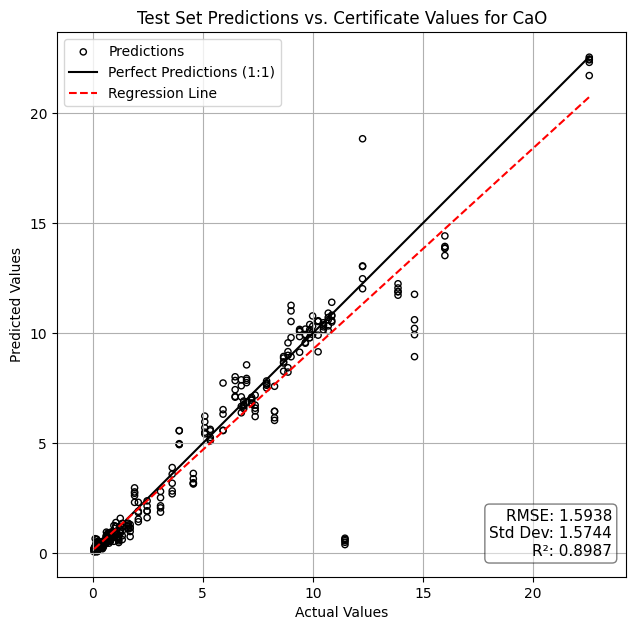
\includegraphics[width=\textwidth]{images/one_to_one/svr/CaO.png}
            \end{subfigure} \\
            \begin{subfigure}{0.5\textwidth}
                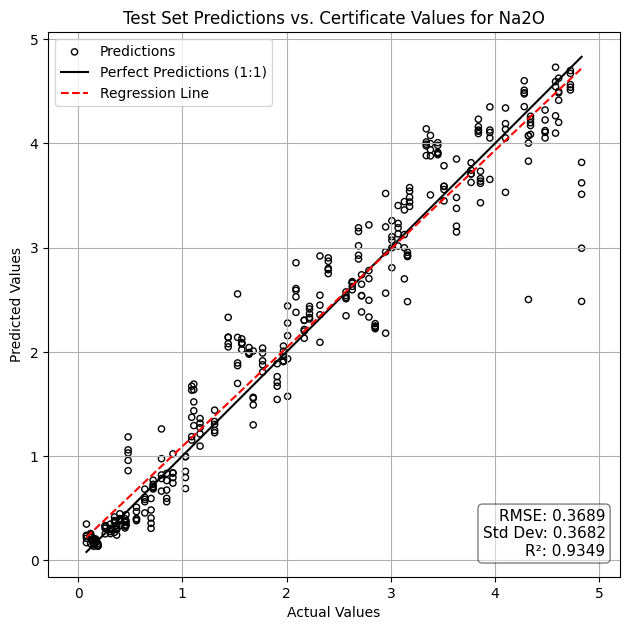
\includegraphics[width=\textwidth]{images/one_to_one/svr/Na2O.png}
            \end{subfigure} & \hspace{3cm}
            \begin{subfigure}{0.5\textwidth}
                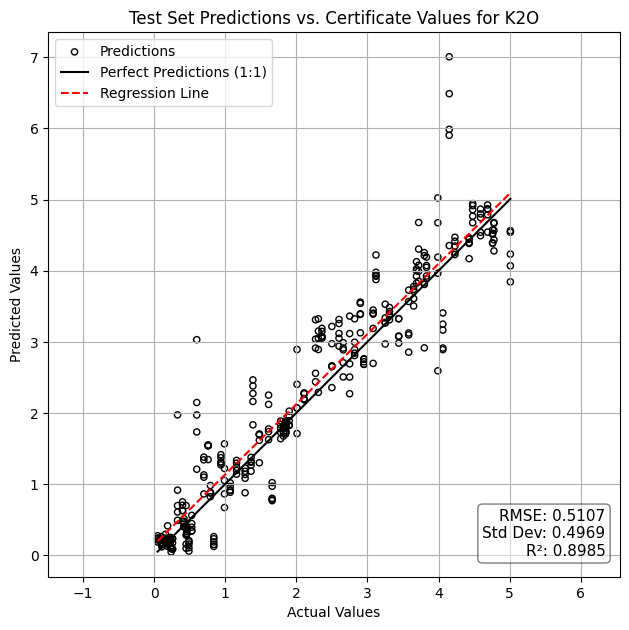
\includegraphics[width=\textwidth]{images/one_to_one/svr/K2O.png}
            \end{subfigure}
        \end{tabular}
    }
    \caption{One-to-one plots for the stacking ensemble model with the \gls{svr} as the meta-learner}
    \label{fig:svr_one_to_one}
\end{figure*}
